\clearpage
\section{Les supernovæ}


%Il a fallut trouver un mécanisme d'introduction d'énergie dans le gaz.
%Les supernoavae ont été proposées comme mécanisme.

Les supernovae ont été introduites dans les simulations cosmologiques pour réduire l'effondrement du gaz sur lui même.
Sans l'introduction d'énergie dans le gaz par les supernovæ, le gaz s'effondre de manière importante et créer un nombre élevé d'étoiles.
Cela mène à un taux de formation stellaire trop important par rapport à ce qui est observé.
Ce problème est connus sous le nom de "overcooling problem" \citep{2003ApJ...599...38B, 1992A&A...264..365B}.
L'objectif est de casser les structures pour diminuer les surdensités et limiter la formation stellaire.

Dans cette section, nous allons aborder la modélisation des supernovæ dans les simulations cosmologiques.
Je présenterai deux des modèles que j'ai implémenté, ainsi que les tests numériques qui vont permettent de les valider.
Nous verrons que ces modèles sont équivalent dans un cas idéal mais divergent lors de l'introduction de la physique du refroidissement.
Nous aborderons également la problématique de la calibration de ces modèles.


%\subsection{Le modèle théorique}
%Il existe principalement deux événement pouvant mener a un explosion de supernovæ : 
%
%\begin{itemize}
%\item soit l'étoile est a l'origine suffisamment massive (plus de 8Mo) pour s'effondrer a la fin de sa vie.
%\item soit l'étoile n'est pas suffisamment massive (elle va donc mourir en naine blanche) mais dispose de suffisamment de matière a proximité (généralement étoiles double ou le compagnon pas en phase géante rouge) pour que sa masse augmente avec le temps.
%la matière accreté va faire passer la masse de cette étoile au dessus de la limite.
%\end{itemize}
%
%Les étoiles de plus de 8mo exploses en SN en injectant 1e51 erg dans le milieu\\
%Cette injection limite fortement la formation stellaire dans le milieu.\\
%modèle sous grille\\


\subsection{La mort d'une étoile}
\label{sec:snmort}

Arrivé à un certain taux de consommation d'hydrogène, les réactions protons-protons ne sont plus suffisantes et l'étoile s'effondre sur elle même.
%A la fin de sa vie, une étoile a consommée la plus grande partie de son hydrogène disponible.
L'équilibre entre la gravité et la pression est rompu, ce qui mène à une augmentation de la pression interne.
% Géante rouge ?
Cette augmentation de la pression amorce une nouvelle série de fusions nucléaires, qui va consommer des éléments plus lourds que l’hydrogène, tel le carbone, l'azote ou l'oxygène (cycle CNO) jusqu'au fer où le processus s'arrête.
A ce stade, les couches externes de l'étoiles se contracte rapidement, et rebondissent sur le noyau de fer.
L'étoile explose alors en supernovae et injecte énormément d'énergie dans le milieu, de l'ordre de $10^{51}$ erg par explosion. 
%Une fois arrivé au Fe, il devient coûteux de continuer a fusionner des éléments car Fe est le plus stable.

Il existe principalement deux types de supernovæ : 
\begin{itemize}
\item Les types I où l'étoile n'est pas assez massive à la base pour permettre l'explosion en supernovae.
Ce sont généralement des étoiles binaire où une des deux étoiles accrète une partie de son compagnon, ce qui mène au passage au dessus de la masse limite et provoque l'explosion.
\item Les types II : les étoiles de plus de 8$M_\odot$ sont assez massives pour exploser en supernovæ sans avoir besoin de masse supplémentaire.
\end{itemize}

Pendant l'explosion, l'énergie libérée est suffisamment importante pour amorcer la formation d'éléments plus lourds que le fer.
Ces éléments, ainsi que ceux formés pendant la vie de l'étoile vont être expulsés, et vont participer à l'enrichissement du milieu.
Ce qui va changer les propriétés physico-chimiques du gaz environnant et avoir des conséquences sur la formation des prochaines générations d'étoiles.

Après l'explosion de la supernova, le cœur subsiste et en fonction de sa masse, plusieurs scénario d'évolution sont possibles.
En fonction de la masse de l'étoiles, le résidu peux devenir une naine blanche, une étoile à neutron ou un trou noir.
Dans tout les cas, le résidu continue à interagir gravitationnellement avec son environnement.

%\begin{itemize}
%\item Naine blanche %(maintenue par le pression de dégénérescence des électrons)
%\item Étoile a neutron %(pression de dégénérescence des neutrons)
%\item Trou noir %(singularité)
%\end{itemize}


\subsection{Les différentes phases}
Après l'explosion d'une supernovae, il en résulte une onde de choc qui va se propager dans le milieu environnant.
L'évolution du front d'onde a lieu en plusieurs phases, on en distinguera principalement deux : 

\begin{itemize}
\item Expansion adiabatique.
Dans la phase d'expansion adiabatique, l'énergie cinétique est conservée, le choc est violent et le gaz n'a pas le temps de perdre de l'énergie par radiation.
Dans cette phase, le front d'onde est suffisamment rapide pour que la dissipation d'énergie par radiation soit négligeable.
%C'est par exemple le cas du test de Sedov.

\item Snowplow.
Dans la phase snowplow, le choc a suffisamment ralentis pour que le gaz commence à dissiper de l'énergie par rayonnement.
Dans ce cas, il se forme un bourrelet de compression dans lequel le gaz est poussé, comme dans le cas d'un chasse neige. 
Les pertes par radiation deviennent importantes et l'énergie cinétique n'est plus conservée.
\end{itemize}

\subsection{Les Superbubbles}
%A la manière de la percolation des bulles de HII, les bulles de supernovae 

Dans les lieux de formation stellaire, les étoiles ne sont pas isolées, mais apparaissent ensemble au sein d'un même nuage de gaz.
L'effondrement gravitationnel du nuage mène à créer une génération d’étoiles en un cours laps de temps.
Toutes ces étoiles vont mourir dans un court délai et les différentes supernovæ vont injecter de l’énergie dans le milieu en même temps.
Les différentes ondes de chocs vont se cumuler et la résultante va mener à la création d'une bulle de gaz chaud pouvant englober les galaxies.
On appelle ces régions des superbubbles.

\subsection{Considérations d'échelles}
La façon de gérer les supernovæ sera donc fonction de l'échelle que l'on considère.
Dans des simulations détaillées de galaxies, il sera nécessaire de résoudre la phase adiabatique des explosions d'étoiles individuelles. %TODO ref simu de galaxie zoom
Dans les simulations cosmologiques de la réionisation qui nous intéresses ici, l’intérêt sera plus porté sur la phase snowplow des superbubbles.

%\subsection{ Différentes implémentations existantes}
%\subsubsection{Navaro and white}
%\subsubsection{Stinson et al}
%\subsubsection{dubois et Teyssier}
%Utilisation de particule fantômes pour simuler les différentes phase
%
%\subsubsection{Dalla Veccia et Schaye}
%Modèle probabiliste, injection d'énergie seulement si l'énergie est suffisante pour générer un mouvement suffisant.

\subsection{Mes Implémentations}
\label{sec:SNmodel}

\subsubsection{Modèle thermique}
Le modèle thermique consiste à injecter l’énergie de l'explosion sous forme d’énergie interne.
Il existe 2 variables d’état liées à l’énergie interne : la pression et la température.
Modifier l'une ou l'autre est équivalent et dans l’implémentation actuelle, le choix a été fait de travailler sur la pression.
Elle est modifiée de la façon suivante :

\begin{equation}
P^{0+} = P^{0-}  + E_{SN} \cdot  (\gamma-1)
\end{equation}
où $E_{sn}$ représente l'énergie à injecter et $\gamma$ l'indice adiabatique du gaz.

L'injection de l'énergie va donc résulter en une augmentation de la pression dans la cellule et le gaz sera mis en mouvement par conversion de l'énergie interne en énergie cinétique. 
L'avantage de cette méthode est que l'injection ne nécessite la modification que d'une seule cellule.
Cependant il est connu pour avoir de fortes pertes de d'énergie dans le cas ou le refroidissement est autorisé \citep{navarro_simulations_1993}. 

\subsubsection{Modèle cinétique}

Le modèle cinétique a pour objectif d'éviter le conversion entre énergie interne et énergie cinétique en modifiant directement cette dernière.
Le modèle cinétique consiste à modifier directement la vitesse du gaz autour de l'explosion dans le but de shunter la conversion de l'énergie interne en mouvement.
%Ce type de model a été utilisé pour 
Il n'est plus possible ici de ne modifier qu'une seule cellule.
Plus le nombre de cellules dont la vitesse sera modifiée autour de l'explosion sera important, meilleure en sera la sphéricité de l'onde choc.
Le choix a été fait de limiter le nombre de cellules utilisées à 8 correspondant à 1 oct de la structure \ac{AMR} d'\emma .
Ceci à deux conséquences.
Premièrement la recherche de voisin est réduite à l'exploration de l'OCT parent de la cellule ou a lieu l'explosion, le coût numérique est donc réduit à son strict minimum (voir section \ref{sec:voisins}).
Deuxièmement, un OCT ne peut pas être divisé entre les processus, ce qui assure que l'explosion a lieu au sein d'un processus unique et permet d'éviter les communications.

En pratique l'énergie de l'explosion sera uniformément répartie sur les 8 cellules de l'OCT, ainsi chaque cellule recevra : 

\begin{equation}
e_{SN} = E_{SN}/8.
\end{equation}

Cette énergie est utilisée pour changer la vitesse du gaz de chaque cellule en utilisant : 

\begin{equation}
    \Delta \overrightarrow{v_{gas}} = \sqrt{\frac{2e_{SN}}{\rho_g.dV}} \overrightarrow{u}
    \label{eq_sn_direct}
\end{equation}

Où les vecteurs $\overrightarrow{u}$ sont les directions radiales au centre de l'OCT présentés sur la figure \ref{fig:kin}.

\begin{figure}
        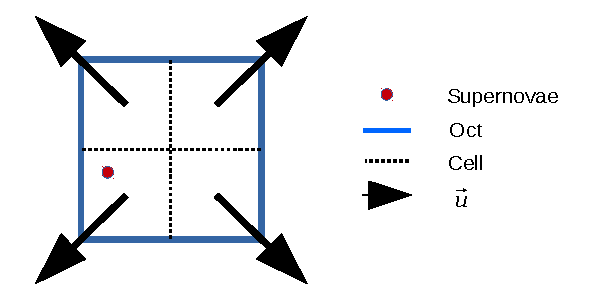
\includegraphics[width=.95\linewidth]{img/03/oct_kinetic.pdf} 
        \caption[Injection d'énergie cinétique]{Avec le modèle cinétique l'explosion a lieu au sein d'un OCT, et radialement au centre de celui ci.
 		\label{fig:kin}}
\end{figure}

\subsection{Retour de masse}
Les deux modèles présentés ont la possibilité de retourner de la masse dans le milieu environnant après l'explosion.
La totalité de la masse sera retournée dans une cellule dans le cas du modèle thermique, ou uniformément distribuée dans les 8 cellules de l'OCT dans le cas du modèle cinétique.
En pratique la densité de la cellule sera modifiée:
\begin{equation}
\rho^{0+} = \rho^{0-} + \frac{M_{SN}}{dV}
\end{equation}
L’enrichissement en métaux (cf section \ref{sec:snmort}) n'est pas considéré actuellement, mais fait partie des améliorations planifiées.

\subsection{Test numérique - Explosion de Sedov}
\label{sec:sedov}

%la dérivation des solutions du test de Sedov se trouve :
%chapitre 17 de Shu the physique of astrophysic Volume 2.\\

Dans le but de tester l'implémentation des différents modèles d'injection d'énergie, je les ai soumis au test de Sedov.
Ce test est utilisé pour tester le cas d'une explosion parfaite et a l'avantage de posséder une solution analytique.
Il consiste à relâcher instantanément une quantité d'énergie $E_0$ dans un milieu homogène d'indice adiabatique $\gamma$, de densité $\rho_0$ et de pression $P_0$ (ou de température $T_0$).
Ce brusque changement dans l'état du système créer une discontinuité que le solveur va devoir gérer.
\cite{sedov_similarity_1959} a exprimé le rayon de l'explosion en fonction du temps  : 

\begin{equation}
r_{(t)}=\left( \frac{E_0}{\alpha \rho_0 }\right)^{1/5} t^{2/5}
\end{equation}

%TODO expression analytique du profil

\subsubsection{Évolution temporelle }

%parametre du test :
%rho=1
%p=1e-5
%v=0
%gamma=5/3

Ce premier test consiste à injecter l'énergie dans le milieu et à suivre l'évolution du profil et de la position de l'onde de choc dans le temps.
%On s'assure alors que son profil et sa position sont correct 
%On calcul pour chaque cellule sa distance au centre de l'explosion, puis en utilisant un histogramme sur les rayons, pondéré par la valeur du champ que l'on veux analyser, on obtient rapidement le profil radial moyen.

La colonne de gauche de la figure \ref{fig:sedov_profil} présente les profils radiaux de densité, de pression et de vitesse radiale à trois instant différents, comparé à la solution analytique.
Le résultats présentés utilisent l'injection thermique dans une seule cellule.
Le domaine est une grille régulière décomposée en $256^3$ éléments de calcul et le raffinement n'est pas autorisé.
On observe un très bon accord entre la simulation et la théorie, l'implémentation de la méthode d'injection d'énergie thermique est donc correcte et bien dimensionnée.

\subsubsection{Comparaison des modèles}

Le test présenté ici consiste à vérifier la validité de différentes méthodes d'injection, nous allons en comparer trois : 
\begin{itemize}
\item l'injection thermique dans une cellule,
\item l'injection thermique dans un cube de huit cellules,
\item l'injection cinétique dans un cube de huit cellules.
\end{itemize}

Les trois simulations utilisent cette fois ci un espace discret de $128^3$ éléments, mais en autorisant le raffinement sur 3 niveaux.
Dans le but de concentrer le raffinement sur le front de l'onde choc, le raffinement est effectué sur le gradient de densité : une cellule est raffinée si son gradient de densité est supérieur à un seuil donné (la valeur de ce seuil est déterminée de manière empirique).

La colonne de droite de la figure \ref{fig:sedov_profil} présente les profils obtenus à un instant donné pour les différentes méthodes d'injection d'énergie et pour les différents champs.
On observe que le front est bien situé au même endroits indépendamment de la méthode et que les profils sont globalement identiques excepté quelques différences au centre.
%Le profil de densité est présenté en échelle logarithmique pour accentuer les difference au niveau du centre. 

Même si les profils radiaux moyens sont comparables, on observe des différences sur la forme de l'explosion.
La figure \ref{fig:sedovslice} présente une coupe suivant l'axe $z$ de la grille, contenant la cellule d'injection, pour les trois méthodes.
Ces différences sont dues à la grille et à la façon dont les flux sont calculés.
Dans le cas de l'injection thermique, les flux auront tendance à être suivant les axes principaux de la grille, donnant ce motif en forme de "+" bien particulier.
Dans le cas de l'injection cinétique, les vitesses sont forcées à être dans des directions obliques, à 45° par rapport à la l'axe de la grille, donnant cette fois si une figure en forme de "x".
Le panneau inférieur droit de la figure \ref{fig:sedovslice} présente le motif de raffinement obtenu pour le test d'injection thermique sur une cellule.
Le motif de raffinement est similaire pour les trois simulations.

\begin{figure}
   \begin{minipage}[c]{.5\linewidth}
        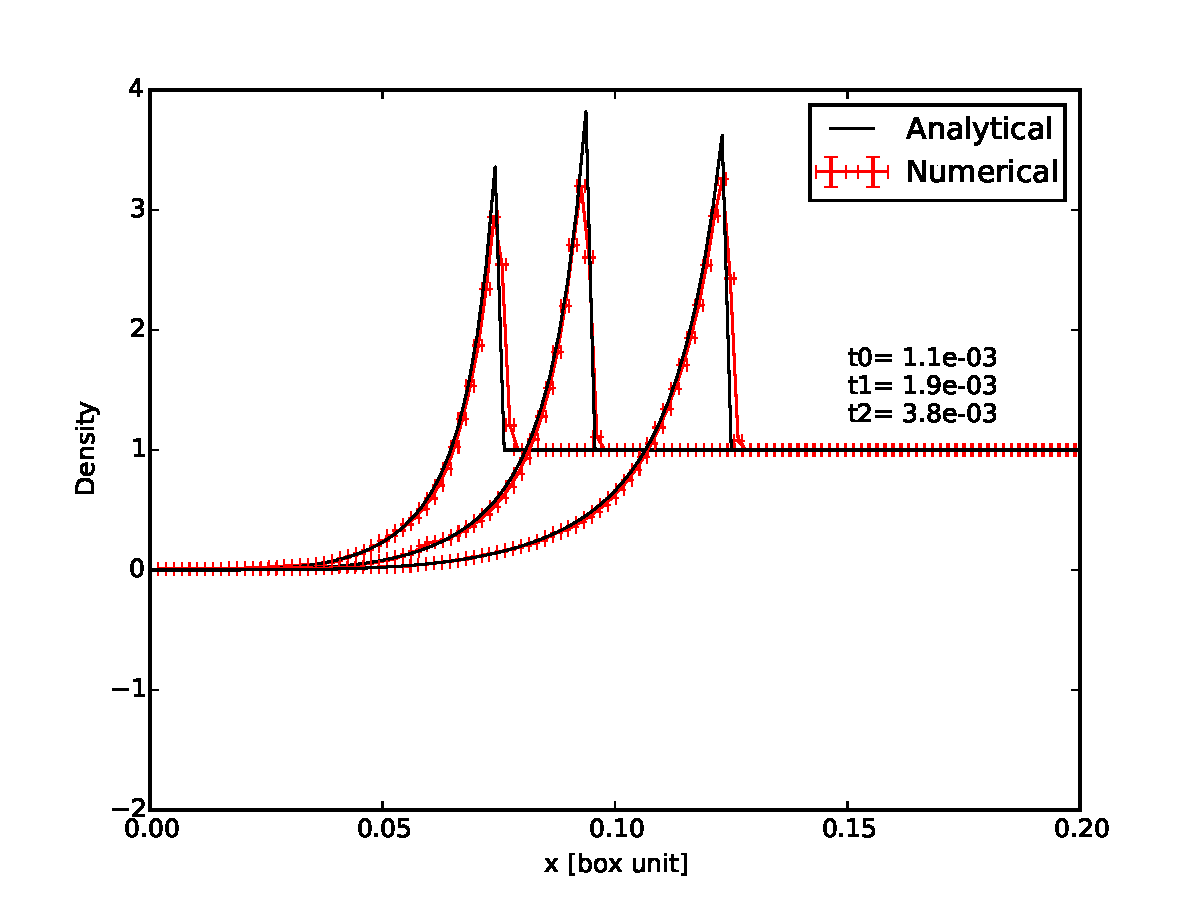
\includegraphics[width=\textwidth]{img/03/sedov/sedov_evol_8_den_lin.pdf} 
		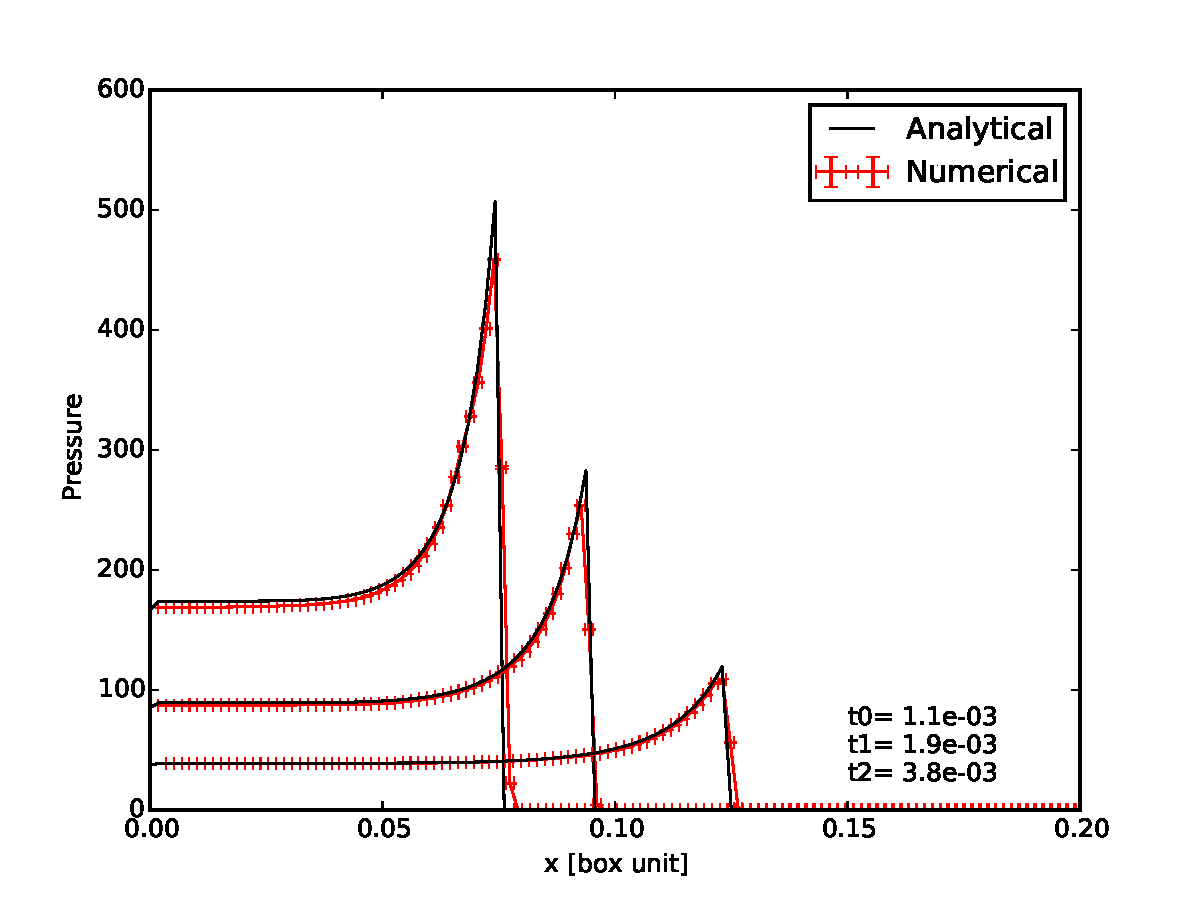
\includegraphics[width=\textwidth]{img/03/sedov/sedov_evol_8_pres.pdf} 
		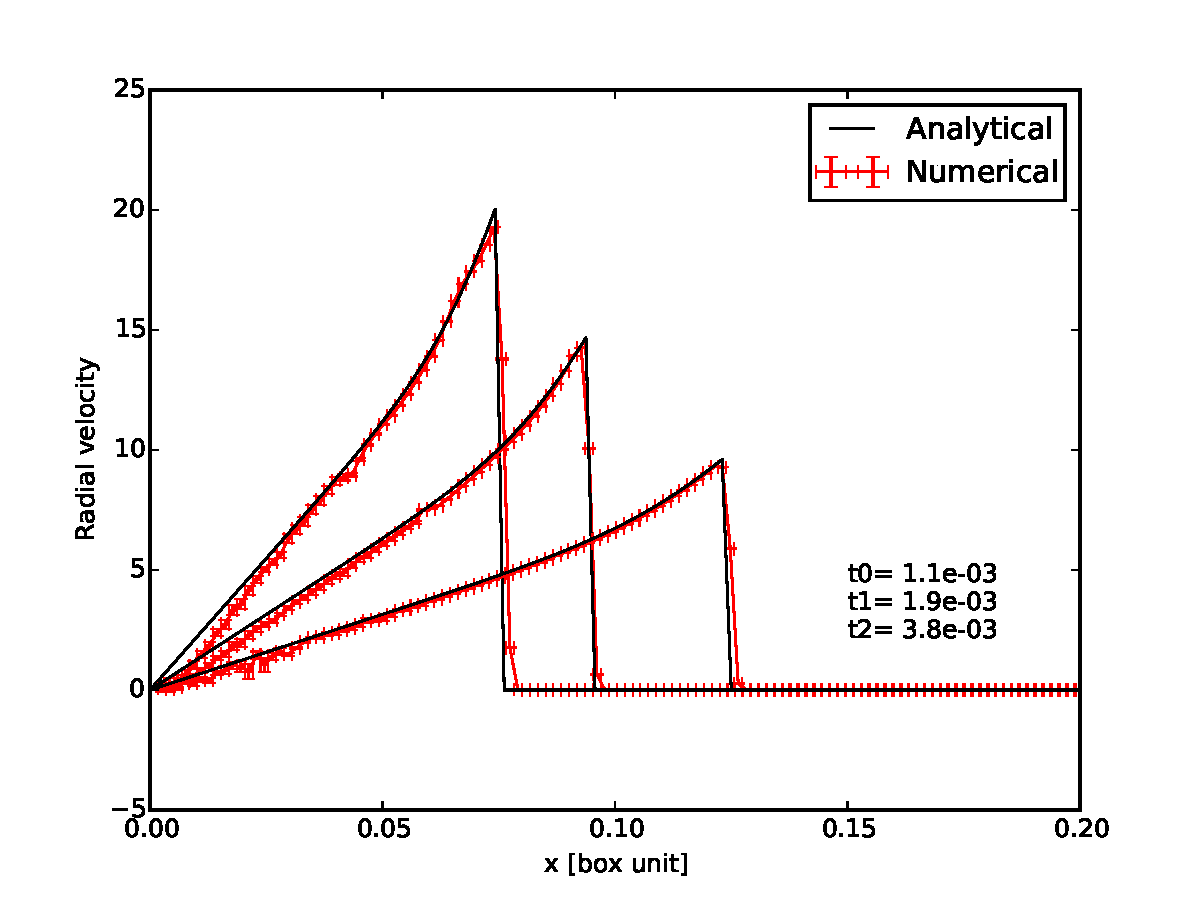
\includegraphics[width=\textwidth]{img/03/sedov/sedov_evol_8_vel.pdf} 

   \end{minipage} \hfill
   \begin{minipage}[c]{.5\linewidth}
		
		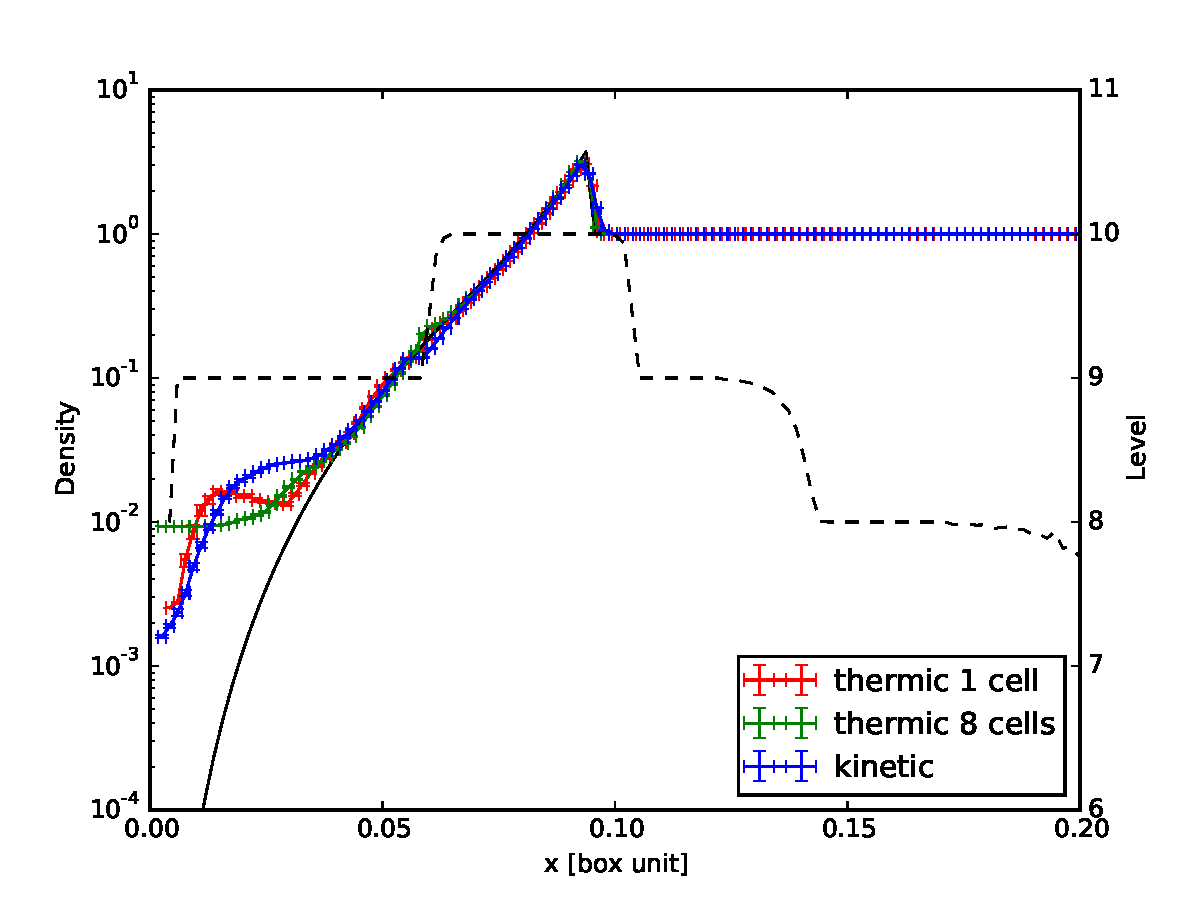
\includegraphics[width=\textwidth]{img/03/sedov/sedov_comp_profile_den.pdf} 
		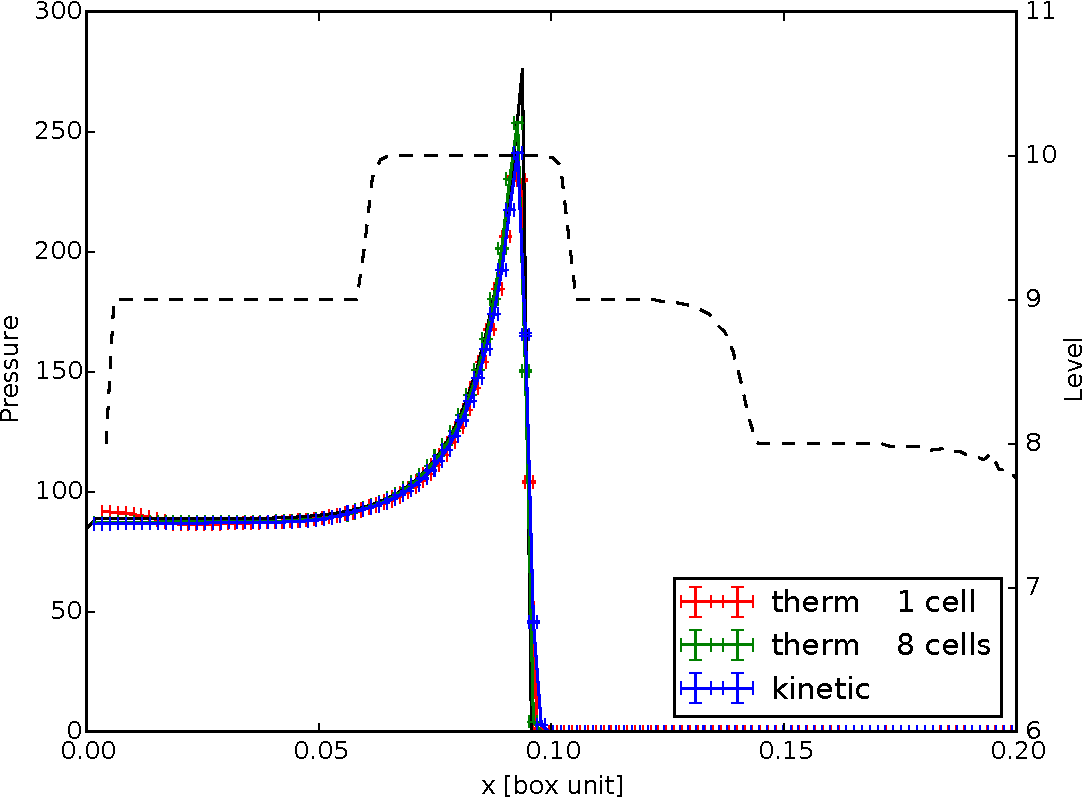
\includegraphics[width=\textwidth]{img/03/sedov/sedov_comp_profile_pres.pdf} 
		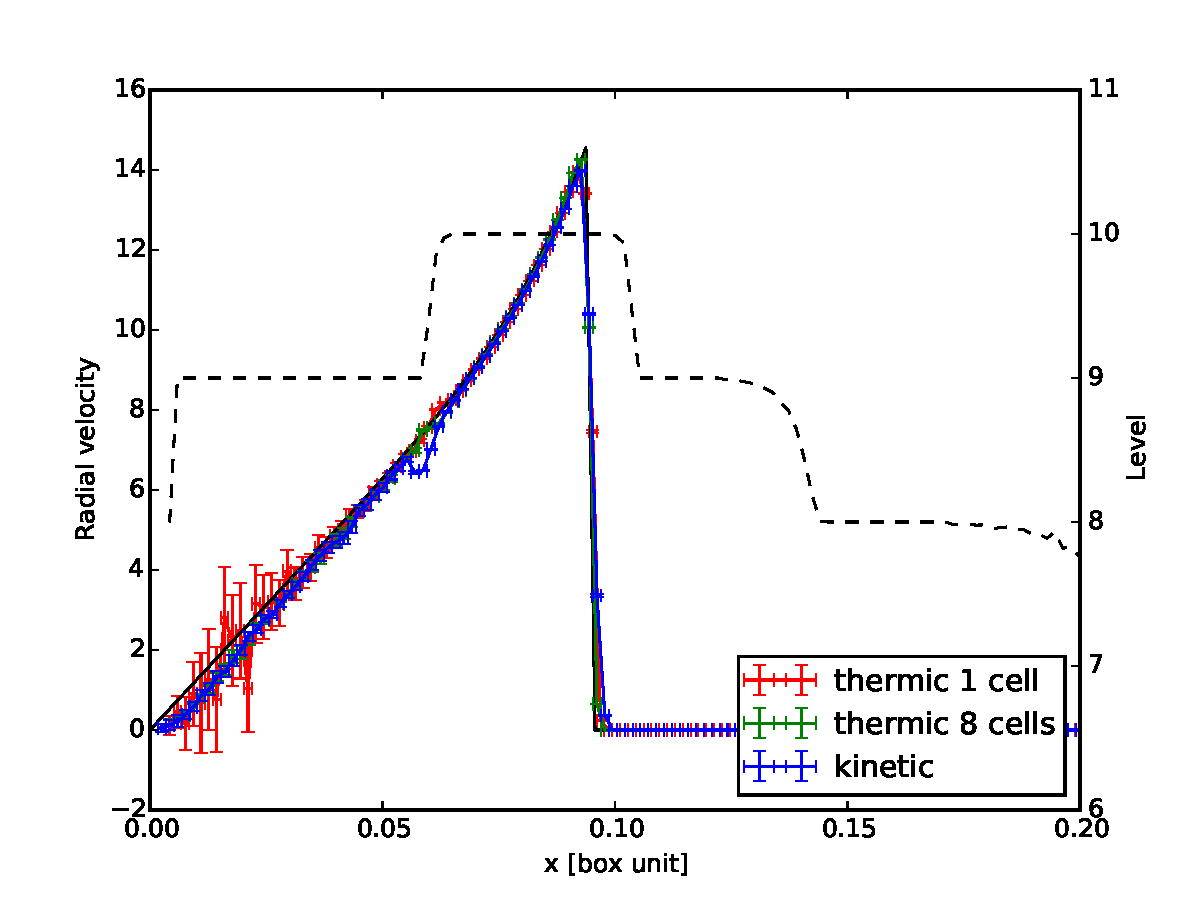
\includegraphics[width=\textwidth]{img/03/sedov/sedov_comp_profile_vel.pdf} 

   \end{minipage}

        \caption[Test de Sedov - Profils]{Profils radiaux des différentes variables d'états lors du test de Sedov, . 
        La densité en haut, la pression au milieu et la vitesse radiale en bas.     
        Colonne de gauche :
        Comparaison des profils à différents instants avec le méthode d'injection thermique.
        L'accord avec la théorie est excellent.
        Colonne de droite :    
        Comparaison en fonction des méthodes d'injection. 
        La position et la forme du front d'onde ne dépendent pas de la méthodes d'injection utilisée.
 		\label{fig:sedov_profil}
 		}
\end{figure}

\begin{figure}

	\centering
	\subfloat[]{ 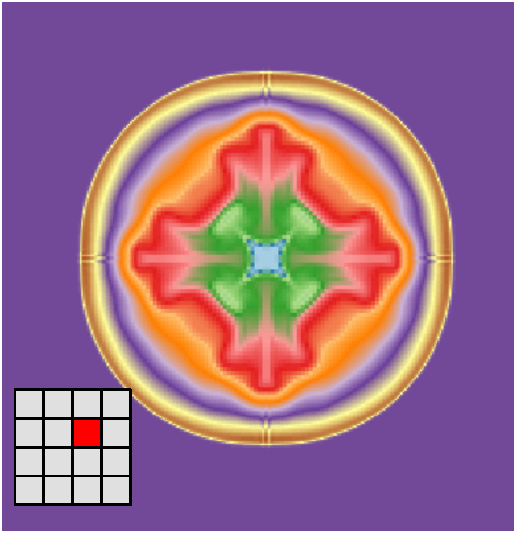
\includegraphics[width=.45\linewidth]{img/03/sedov/slice_therm1.pdf}} 
	\subfloat[]{	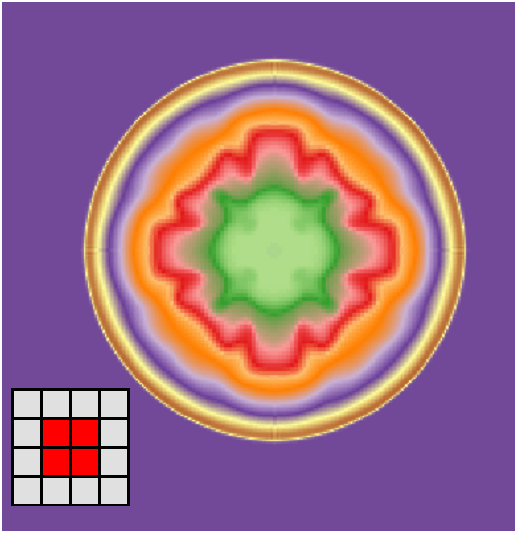
\includegraphics[width=.45\linewidth]{img/03/sedov/slice_therm4.pdf}} \\

	\subfloat[]{	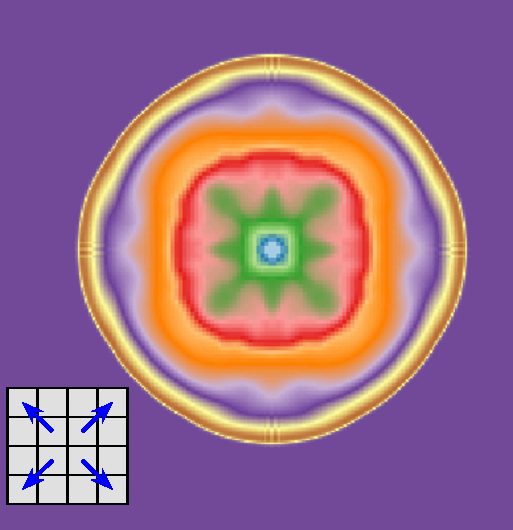
\includegraphics[width=.45\linewidth]{img/03/sedov/slice_kin.pdf} }
	\subfloat[]{	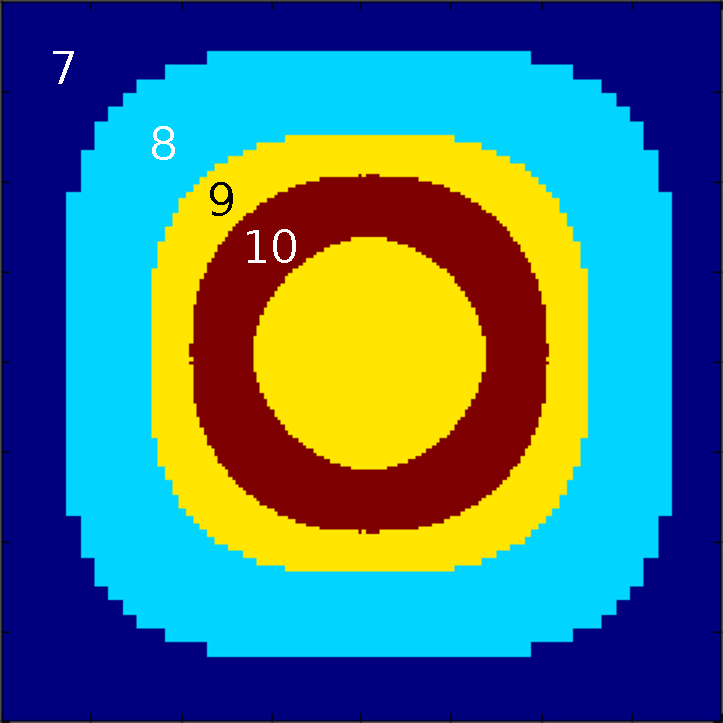
\includegraphics[width=.45\linewidth]{img/03/sedov/slice_th_1raf_cut.pdf}}

    \caption[Test de Sedov - Tranches]{Différents motif d'explosion en fonction de la méthodes d'injection.
    Chaque figure représente une tranche d'une cellule d'épaisseur contenant le site de l'explosion.
    (a), (b) et (c) représente le champ de densité prit au même instant.
    Dans le but d'accentuer les différence, la représentation utilise le logarithme de la densité avec une colormap quantitative.
    A cause de la grille de calcul, il existe des axes privilégiés pour les flux, il en résulte des motif en croix et ou en losange.
    La figure (d) représente les niveaux de raffinements, l'échelle est différente et le niveau 10 est aligné sur le front d'onde.
    }
 	\label{fig:sedovslice}
\end{figure}

\subsection{Calibration}
\label{sec:sncali}
La quantité d'énergie et de masse injectée est calibrée en utilisant les informations en sortie de Starburst99.
Le modèle actuel ne considère pas la possibilité d'une explosion continue, avec un retour de masse ou d'énergie s'étalant dans le temps.
L'injection est réalisée instantanément quand la quantité d’énergie théorique donnée par Starburt99 représente 50\% de l’énergie totale.
La comparaison entre les sorties de Starburst99 et le modèle implémenté est présenté sur la figure \ref{fig:SNloss}.
Dans ce modèle, un particule stellaire injectera $E_{SN} = 9.7\cdot 10^{11} J.kg^{-1}$ et perdra 53\% de sa masse dans le milieu environnant, $17.6$ millions d'années après sa formation.
On notera que le temps d'explosion des supernovae est environs quatre fois plus grand que le temps de vie radiatif.

De plus on introduira le rendement énergétique des supernovae $\epsilon_{SN}$, ce paramètre libre sera appliqué à $E_{SN}$ et sera utile pour calibrer l'impact de nos modèles.
A l'instar du paramètre de fraction d'échappement intrinsèque du rayonnement (cf section \ref{sec:etoilerad}) il contient une grande partie de la physique sous grille qui n'est pas modélisée ici.

\begin{figure}
        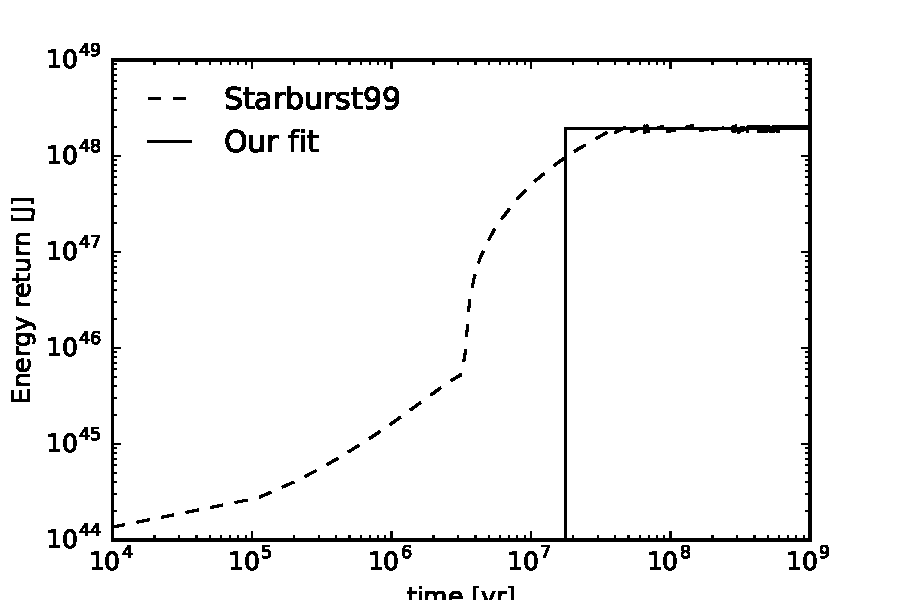
\includegraphics[width=.95\textwidth]{img/03/energy_loss.pdf} 
		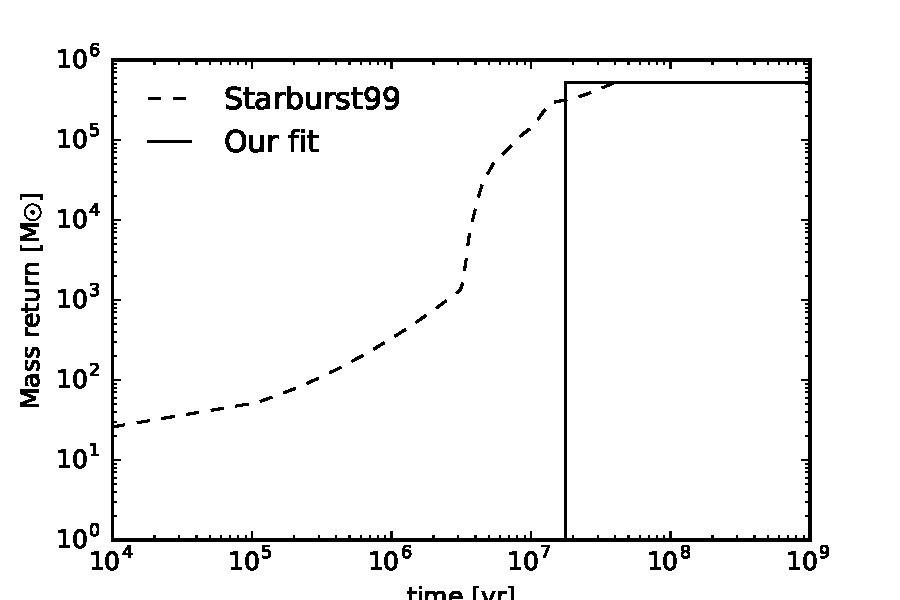
\includegraphics[width=.95\textwidth]{img/03/mass_loss.pdf} 
        \caption[Calibration des supernovæ]{ Quantité d'énergie et de masse injectés par les supernovae. 
        Comparaison entre le modèle théorique de Starburst99 et le modèle d'injection instantané implémenté dans EMMA.
 		\label{fig:SNloss}}
\end{figure}


\clearpage
\section{Tests du modèle en conditions de production}

L'objectif de cette section est de présenter quelques tests pour valider le modèle de formation et d'évolution stellaire développé dans les sections précédentes.
Dans un premier temps, j'ai réalisé une série de simulations, avec pour objectif d'obtenir une \ac{SFH} et un redshift de réionisation simulé en accord avec les contraintes observationnelles.

%Dans le but de tester ces différentes méthodes d'injections dans un contexte cosmologique j'ai réalisé une série de simulations.
%\subsubsection{Présentation des simulations}
\subsection{Présentation des simulations}
\label{sec:pres_simu}

Les paramètres communs à toutes les simulations qui vont suivre sont les suivants:
Elles représentes un volume de $\left( 8\cdot h^{-1} \mathrm{cMpc} \right)^3$ échantillonnées par $256^3$ éléments de résolutions. % particules de matière noire.
Ce qui mène à une résolution en masse de $3.4 \cdot 10^6 M_\odot$ et une résolution spatiale de $46$ckpc sur le niveau de base.
La grille est raffinée suivant une méthode semi-Lagrangienne (voir Sec. \ref{sec:raffinement}) avec une limite de résolution de 1 kpc.
Les condition initiales ont été générées avec MUSIC \citep{hahn_multi-scale_2011} avec une cosmologie de Planck \citep{planck_collaboration_planck_2016} : 
$\Omega_m=0.3175$, 
$\Omega_v=0.6825$,
$\Omega_b=0.0490$,
$H_0=67.11$,
$\sigma_8=0.830$. 
Les simulations commencent à redshift $z=150$.


\subsection{Test de formation stellaire}

%le premier test réalisé consiste à comparer le \ac{SFR} cosmique de l'ensemble de la boite, aux observations.
Une difficulté est qu'il existe une dégénérescence entre le seuil en densité et l'efficacité de formation stellaire.
En effet, il semble à priori possible d'obtenir des résultats similaire en utilisant, soit un seuil très permissif et une efficacité très faible, ou à l'inverse en ne formant des étoiles que dans les quelques cellules les plus denses avec une efficacité élevée.
Dans la littérature un seuil en surdensité de $\delta_{in}=50\bar{\rho}$ est régulièrement utilisé dans des simulations avec des résolution comparable a celle ci \citep{ocvirk_cosmic_2015,stinson_star_2006}.
L'objectif étant simplement de bloquer la formation stellaire à très haut redshift où le contraste de densité était faible.
J'ai donc fixé ce seuil et ajusté l'efficacité en conséquence.
La figure \ref{fig:test_SFH} présente l'histoire de formation stellaire dans un volume de $\left( 8\cdot h^{-1} \mathrm{cMpc} \right)^3$ obtenue après calibration. 
Les observations sont extraites de \cite{bouwens_reionization_2015}.
%une compilation réalisée par \cite{madau_cosmic_2014}.
L'efficacité de formation stellaire est fixée à $1\%$.
Avec ces paramètres, la \ac{SFH} obtenue respecte les contraintes observationnelles.
Les premières étoiles apparaissent autour du redshift $z\approx 14$, contraint par le paramètre de surdensité.
On observe cependant un saut dans la \ac{SFH} autour de redshift $z=10$ dû à l'enclenchement du dernier niveau de raffinement.

\begin{figure}
        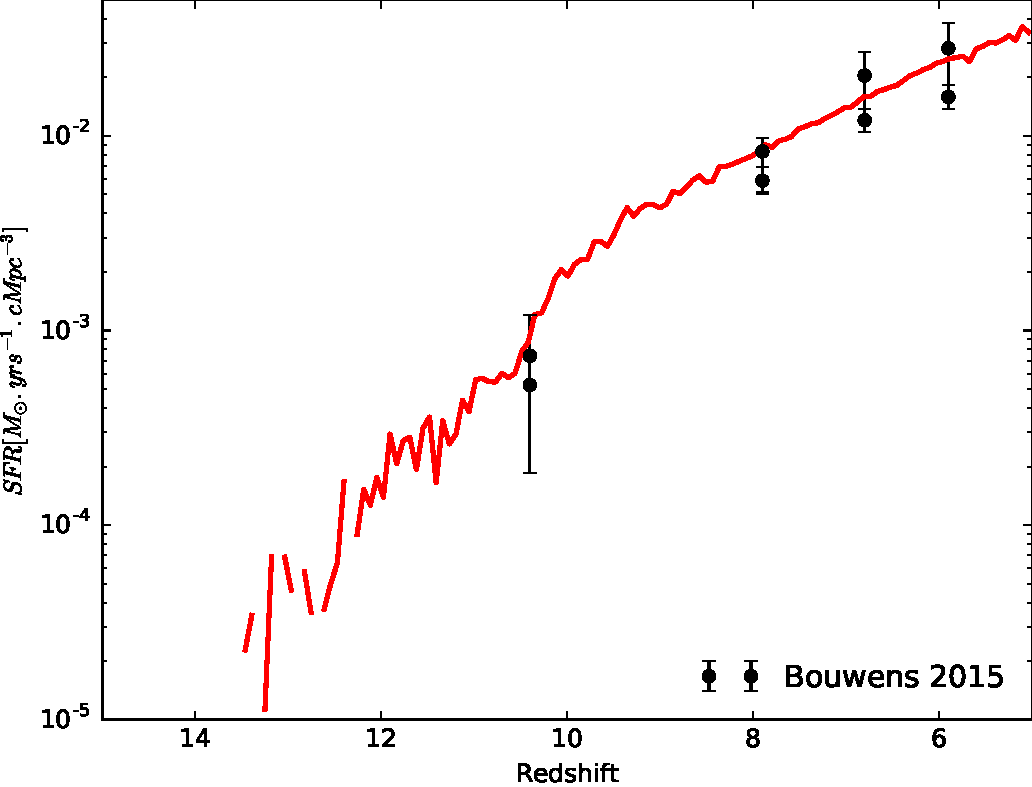
\includegraphics[width=.95\linewidth]{img/02/SFR.pdf}
        \caption[Histoire de formation stellaire]{Histoire de formation stellaire (SFH) d'une simulation de (8/h cMpc)$^3$.
        Il est possible d'obtenir une SFH qui respecte les observations avec un modèle relativement simple.
}
 		\label{fig:test_SFH}
\end{figure}

\clearpage

\subsection{Test radiatif}
Avec les paramètres déterminés par Starburst99 et une fraction d'échappement intrinsèque de 40\%, j'obtiens l'histoire de reionisation présenté sur la figure \ref{fig:test_xion}.
Cette histoire est comparée aux contraintes observationnelles déterminées par \cite{fan_constraining_2006}.
J'ai également pu vérifier à ce stade que l'introduction du rayonnement ionisant dans la simulation a peu d'impact sur la \ac{SFH} cosmique.
Ce qui permet de calibrer d'abord la \ac{SFH} puis ensuite l'émissivité des sources.

\begin{figure}
        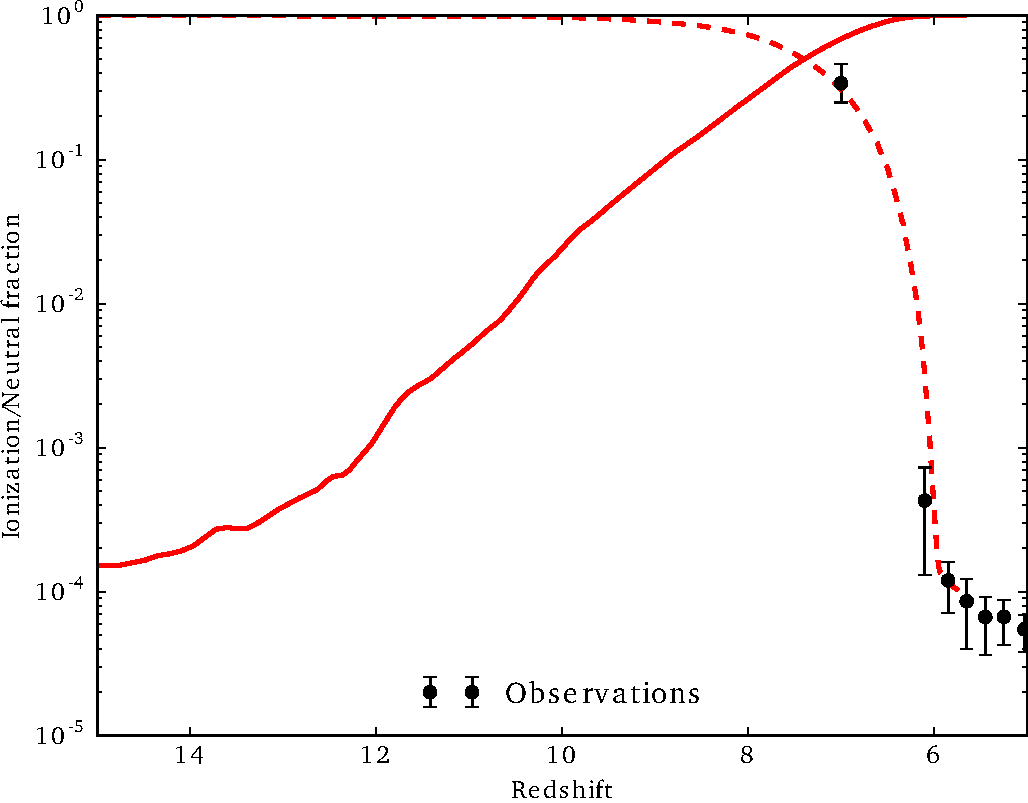
\includegraphics[width=.95\linewidth]{img/02/xion.pdf} 
        \caption[Histoire d'ionisation]{Évolution de la fraction d'ionisation (trais plein) et de la fraction de neutre (tirets) dans la simulation présentée sur la figure \ref{fig:test_SFH}.
        Après calibration de la fraction d’échappement intrinsèque, il est possible d'obtenir une histoire d'ionisation en accord avec les observations.
 		\label{fig:test_xion}}
\end{figure}

\subsection{Le problème de la masse des étoiles}

%le paramètre de masse des étoiles change la reionization\\
%effet numérique\\
%le rayonnement est piégé dans les cellules\\

Durant mes calibrations, il s'est avéré que le paramètre de résolution de la masse des particules stellaire $m_{star}$ avait une grande importance dans l'évolution de la fraction ionisée.
Dans des simulations hydrodynamiques dédiées à l'étude de la formation des galaxies, ce paramètre n'a que peu d'importance.
Il a une faible influence sur la formation stellaire globale (cf panneau de gauche de la figure \ref{fig:mstar}) et ne définira la limite de résolution pour les petits halos.
Dans le cas de simulation \ac{RHD} de l'époque de réionisation, ce paramètre aura également une influence sur la propagation de la radiation.
Même si celui ci n'a pas d'impact sur le \ac{SFR} global, le taux d'ionisation moyen est fortement dépendant de ce paramètre (cf panneau de droite de la figure \ref{fig:mstar}).
Les "grosses" particules stellaire mènent à un taux d'ionisation plus important.
À l'inverse, plus la résolution stellaire est élevée, plus la boite réionise tard.
Il s'agit ici d'un effet numérique lié à la méthode, et pour les plus petites particules stellaires le rayonnement se trouve piégé au sein de la cellule.
Pour les petites particules, le rayonnement est dilué à la fois dans l'espace et dans le temps, alors que dans le cas d'une grosse particule, une grosse quantité de rayonnement est injecté à un instant donné, la cellule est flashée et le rayonnement peut s'échapper.
La difficulté sera de trouver un compromis entre :

\begin{itemize}
\item particules stellaires massives, permettant au rayonnement de sortir facilement des cellules au détriment d'une mauvaise résolution sur la formation stellaire
\item  et particule stellaire de faible masse, générant une formation stellaire résolue même dans les petits halos mais menant à une réionisation plus difficile et une occupation mémoire plus importante.
\end{itemize}

Dans la suite de cette étude, les étoiles seront relativement massive puisque $m_* \approx 7.7 \cdot 10^4 M_\odot$.


\begin{figure}
        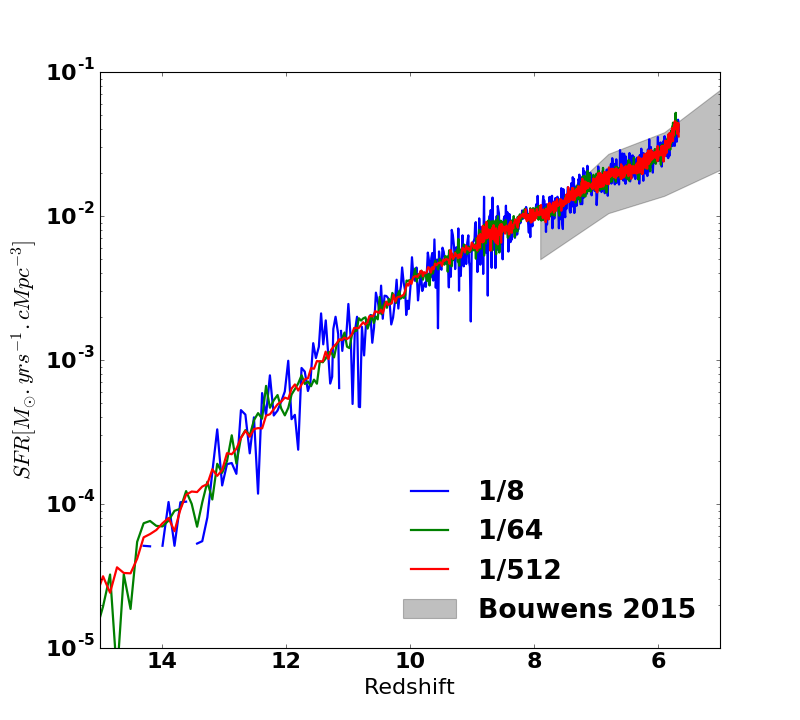
\includegraphics[width=.5\textwidth]{img/02/Mstar_SFH.png} 
        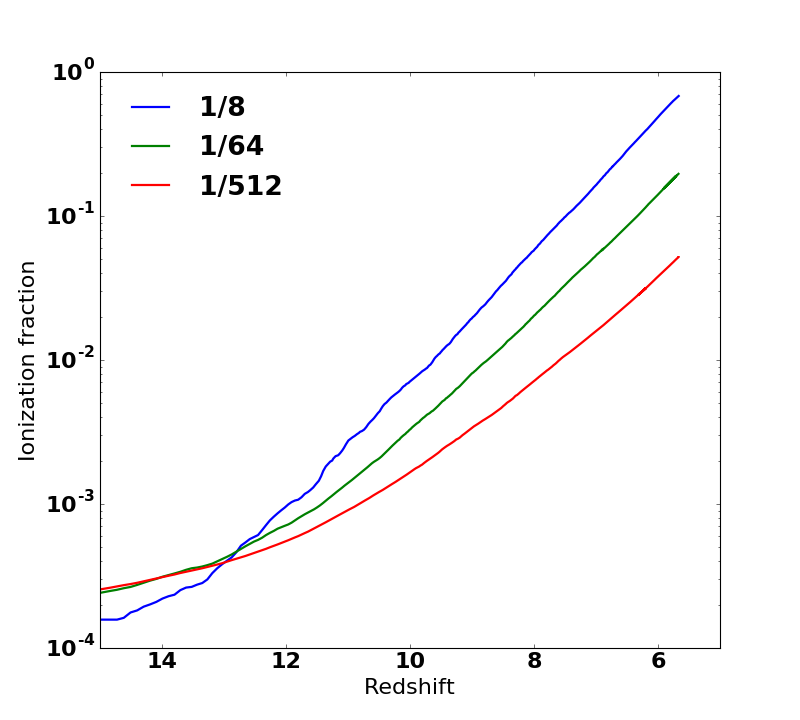
\includegraphics[width=.5\textwidth]{img/02/Mstar_xion.png} 
        \caption[Masse des étoiles]{En changeant le paramètre de résolution en masse des particules stellaire, la \ac{SFH} cosmique moyenne reste constante mais l'histoire d'ionisation s'en trouve impactée.
 		\label{fig:mstar}}
\end{figure}

\clearpage
\subsection{Tests du modèle de supernovæ}


\subsubsection{Influence de la méthode d'injection}
\label{sec:snmethod}

Le premier test consiste à essayer les différents modèle de feedback avec la même quantité d'énergie injectée, et à mesurer leur impact sur la \ac{SFH} cosmique.
Toutes les simulations qui vont suivre sont strictement identiques à l'exception de la méthode d'injection d'énergie.
La figure \ref{fig:sfr_methode} présente les résultats obtenus avec quatre simulations.
Parmi ces simulations, il y en a :
\begin{itemize}
\item une sans rayonnement ni supernovae (NoFEED),
\item une sans supernovae (NoSN),
\item une avec supernovae - modèle thermique (Thermal),
\item une avec supernovae - modèle cinetique (Kinetic).
\end{itemize}

Alors que les deux méthodes présentent des résultats similaires dans le cas idéal, la méthode d'injection cinétique a plus d'impact en conditions cosmologiques.
Ceci est du à l'introduction de la physique du refroidissement.
La méthode thermique repose sur le principe de conversion de l'énergie interne en énergie cinétique, et le refroidissement limite cette conversion en permettant d'importantes pertes par radiation.
La méthode thermique est connue %TODO ref
pour subir d'importante perte d'énergie.
La méthode cinétique outre passe cette conversion et mets directement le gaz en mouvement.
Nous aurons donc tendance préférer la méthode cinétique par la suite, vu que celle ci est plus efficace pour mettre le gaz en mouvement à nos échelles.

%TODO parler du feedback radiatif

\begin{figure}
        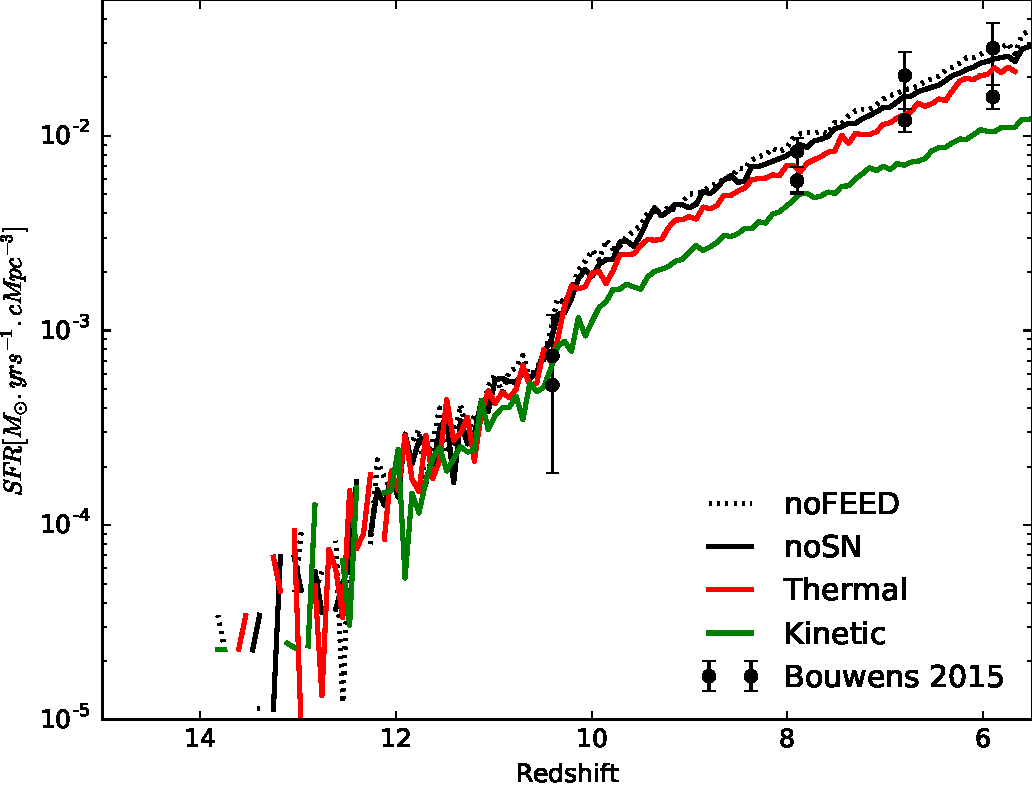
\includegraphics[width=.95\textwidth]{img/03/sedov/SFRmethode.pdf} 
        \caption[SFH cosmique en fonction de la méthode d'injection d'énergie]{SFH cosmique en fonction de la méthode d'injection d'énergie.
        Contrairement au test de Sedov, les différents méthodes n'impactent pas le milieu de la même manière.
        }
 		\label{fig:sfr_methode}
\end{figure}



\subsubsection{Influence de la quantité d'énergie injectée}
\label{sec:snegy}

Le deuxième test consiste à utiliser la méthode cinétique et à varier la quantité d'énergie injectée via le paramètre $\epsilon_{SN}$.
La figure \ref{fig:sfr_egy} présente les résultats obtenus.
On y observe que plus on injecte d'énergie, plus le \ac{SFR} instantané diminue.
Ce qui est le comportement attendus puisque plus les supernovae sont puissantes, plus les sur-densités de gaz sont "cassées", et donc il devient plus difficile de former de nouvelles étoiles.

\begin{figure}
        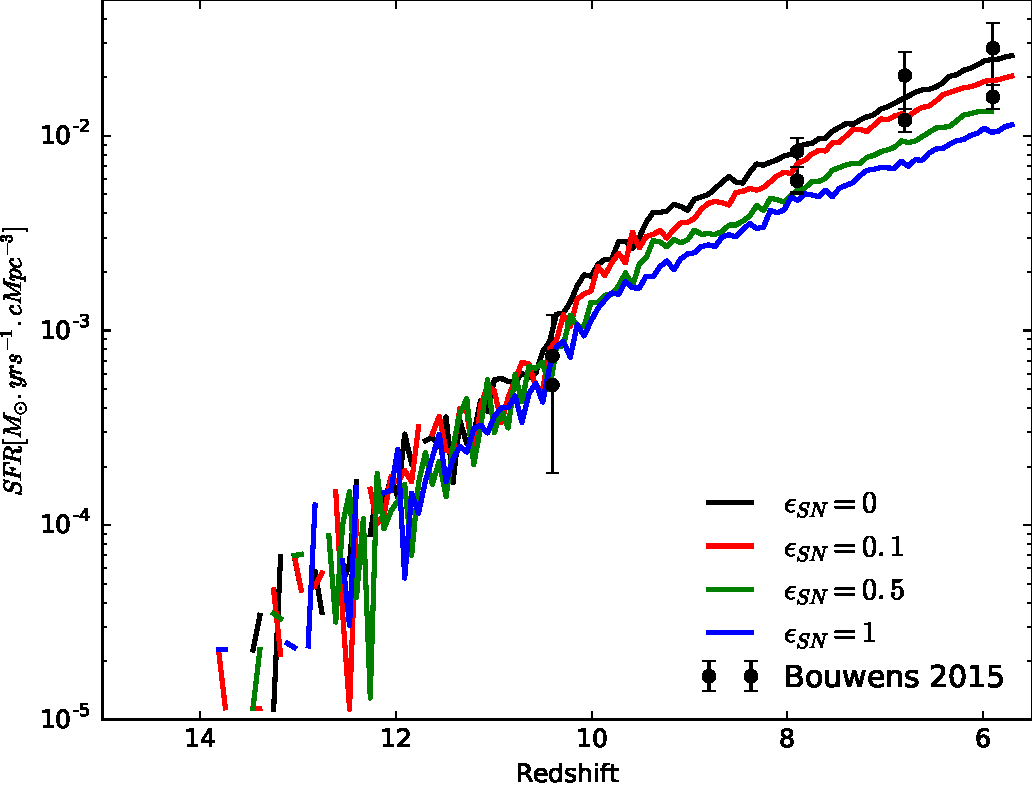
\includegraphics[width=.95\textwidth]{img/03/sedov/sneff_SFR.pdf} 
        \caption[SFH cosmique en fonction de la quantité d'énergie injectée]{SFH cosmique en fonction de la quantité d'énergie injectée. 
        Plus la quantité d'énergie injecté est importante, plus le taux de formation stellaire diminue.
        }
 		\label{fig:sfr_egy}
\end{figure}

\subsubsection{Couplage entre feedback et efficacité de formation stellaire}

Le couplage entre feedback et formation stellaire n'est pas clair et mérite d'être exploré.
En effet, plus on forme d'étoiles et plus le feedback devient important, mais plus il y a de feedback, moins il est facile de former de nouvelles étoiles.

Le troisième test consiste à injecter une quantité donnée d'énergie par supernovae, et à faire varier l'efficacité de formation stellaire.
L'idée est de tester si la diminution du SFR observé lors de l'injection d'énergie peut être compensée par l'augmentation de l'efficacité de formation stellaire.
La figure \ref{fig:sfr_sfe} présente ce test pour trois efficacité de formation stellaire différentes, avec un modèle de feedback cinétique et un rendement énergétique de supernovae de $\epsilon_{SN}=100$ \%.
On observe un fort couplage entre feedback et formation stellaire, à tel point que pour une efficacité de formation stellaire de 10\% le feedback mène à une \ac{SFH} décroissante.
A feedback donné, il n'est donc pas possible de remonter le \ac{SFR} en augmentant l'efficacité de formation stellaire, ce qui limite la dégénérescence entre ces deux paramètres.

\begin{figure}
        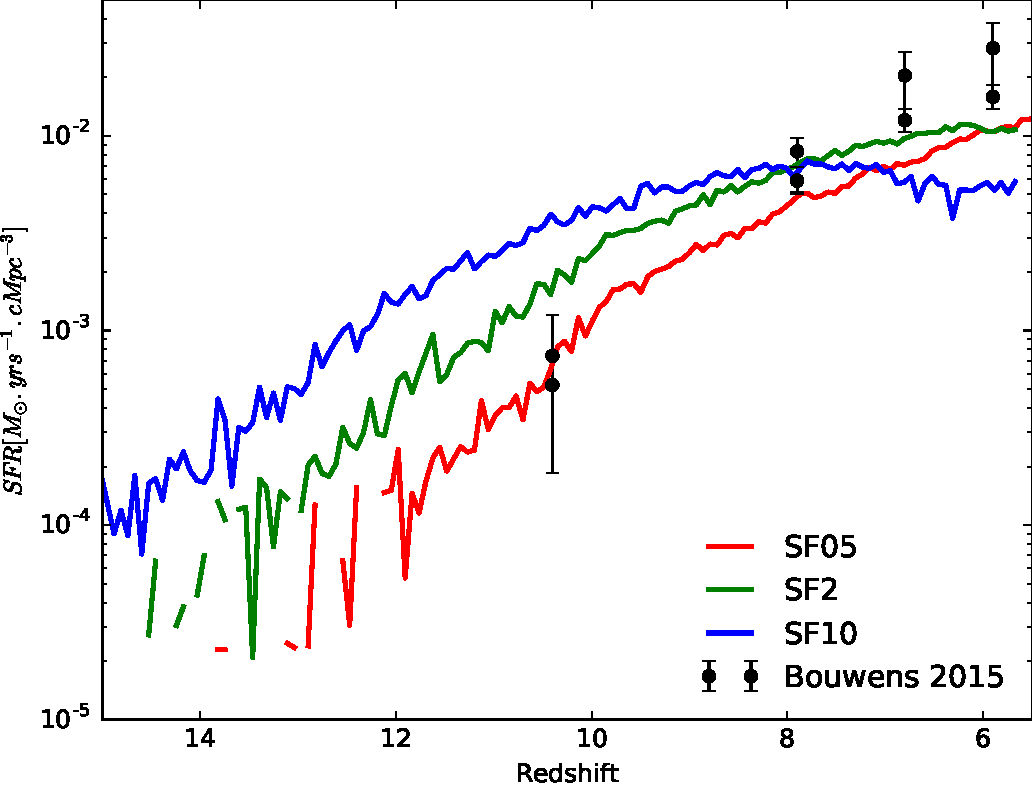
\includegraphics[width=.95\textwidth]{img/03/sedov/SFR_sfeff.pdf} 
        \caption[SFH cosmique en fonction de l'efficacité de formation stellaire]{SFH cosmique en fonction de l'efficacité de formation stellaire.
        Toutes les simulations utilisent la même méthode d'injection et la même quantité d'énergie.
		L'effet du couplage est bien présent.
        }
 		\label{fig:sfr_sfe}
\end{figure}

\subsubsection{Impact sur la fraction d'ionisation}
\label{sec:pbfesc}
Une observation importante par rapport au deuxième test est qu’indépendamment de la quantité d'énergie injectée, et que même si le \ac{SFR} est significativement impacté, l'histoire d'ionisation reste quasiment inchangée (cf figure \ref{fig:xion_sneff}).

Cet effet est inattendu car si la quantité d'étoiles diminue, la quantité de radiation diminue d'autant, et donc la fonction d'ionisation globale devrait être impactée.
Or ce n'est pas ce qui est observé ici.
Dans le but d'explorer cet effet, nous allons nous concentrer dans la suite sur une étude galaxies par galaxies.

\begin{figure}
        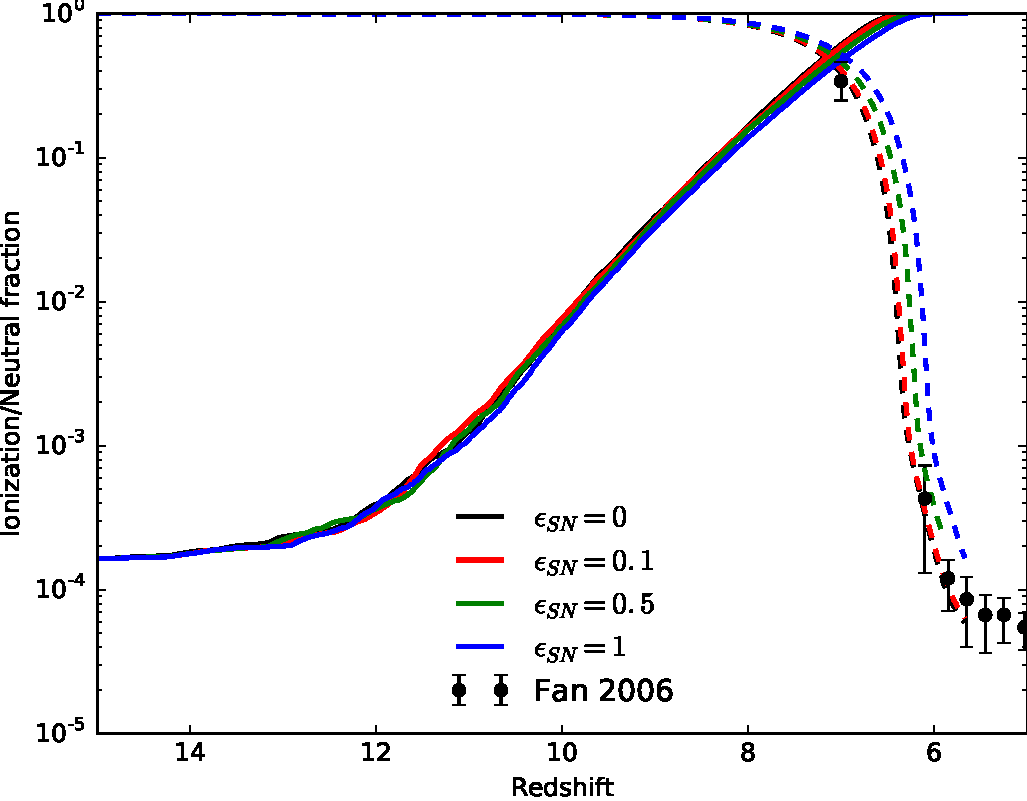
\includegraphics[width=.95\textwidth]{img/03/sneff_xion.pdf} 
        \caption[Fonction d'ionisation en fonction de la quantité d'énergie injectée]{Malgré une SFH différente (voir figure \ref{fig:sfr_egy}), l'histoire d'ionisation est conservée en changeant la quantité d'énergie injectée.
        }
 		\label{fig:xion_sneff}
\end{figure}




%\subsubsection{Conclusion}
%
%La conclusion de ses tests est que les différentes méthodes d'injection sont équivalentes, au moins dans le contexte du test de Sedov.
%OK\\
%mais pas en cosmo
%le pas de temps\\